\documentclass[main.tex]{subfiles} % Subfile-Class


% ============================================================================== %
%                            Subfile document                                    %
% ============================================================================== %

\begin{document}

% Template

\subsubsection{Abstandssensoren}

Wie die Konzeption der Abstandssensoren (siehe
Anhang~\ref{appendix:Hindernisserkennung}) ergeben hat, wird die Detektion der
Umwelt beim ersten Prototyp redundant ausgeführt, welche im Nachfolgemodul dann
noch genauer ausgearbeitet werden.

Das in PREN1 ausgearbeitete Konzept sieht vor, anhand eines LIDAR über die
Hindernisse hinweg den Abstand zu potenziellen Pylonen zu detektieren. Sind
diese näher als 2 m - ist die betrachtete Strecke wahrscheinlich nicht
befahrbar. Ein zweiter Distanzsensor, welcher über Ultraschall arbeiten wird,
detektiert Hindernisse, welche sich näher als $0.5 m$ befinden. Dadurch kann
das Fahrzeug frühzeitig abgebremst werden. Wird die beim Greifer positionierte
Lichtschranke ausgelöst, kann mit Sicherheit davon ausgegangen werden, dass das
Fahrzeug nun beginnen kann und soll, das Hindernis zu greifen und
umzupositionieren.

Diese Funktion könnte allerdings auch vom Ultraschallsensor übernommen werden,
dies wird im Folgemodul weiter untersucht. Ebenfalls befindet sich auf dem
Fahrzeug eine Kamera, welche die vorliegenden Streckenpunkte analysieren kann.
Mit eben dieser Kamera könnten ebenfalls Hindernisse detektiert werden, was
allerdings auch erst im Folgemodul, wenn ein erster Prototyp aufgebaut wurde,
weiter untersucht wird.

\paragraph{Fazit} Das in Abbildung~\ref{fig:Konzept_Hinderniserkennung} gezeigte Konzept stellt
den aktuellen Stand der Entwicklung dar und ist so für den ersten Aufbau
eingeplant.


\begin{figure}[H]
    \centering
    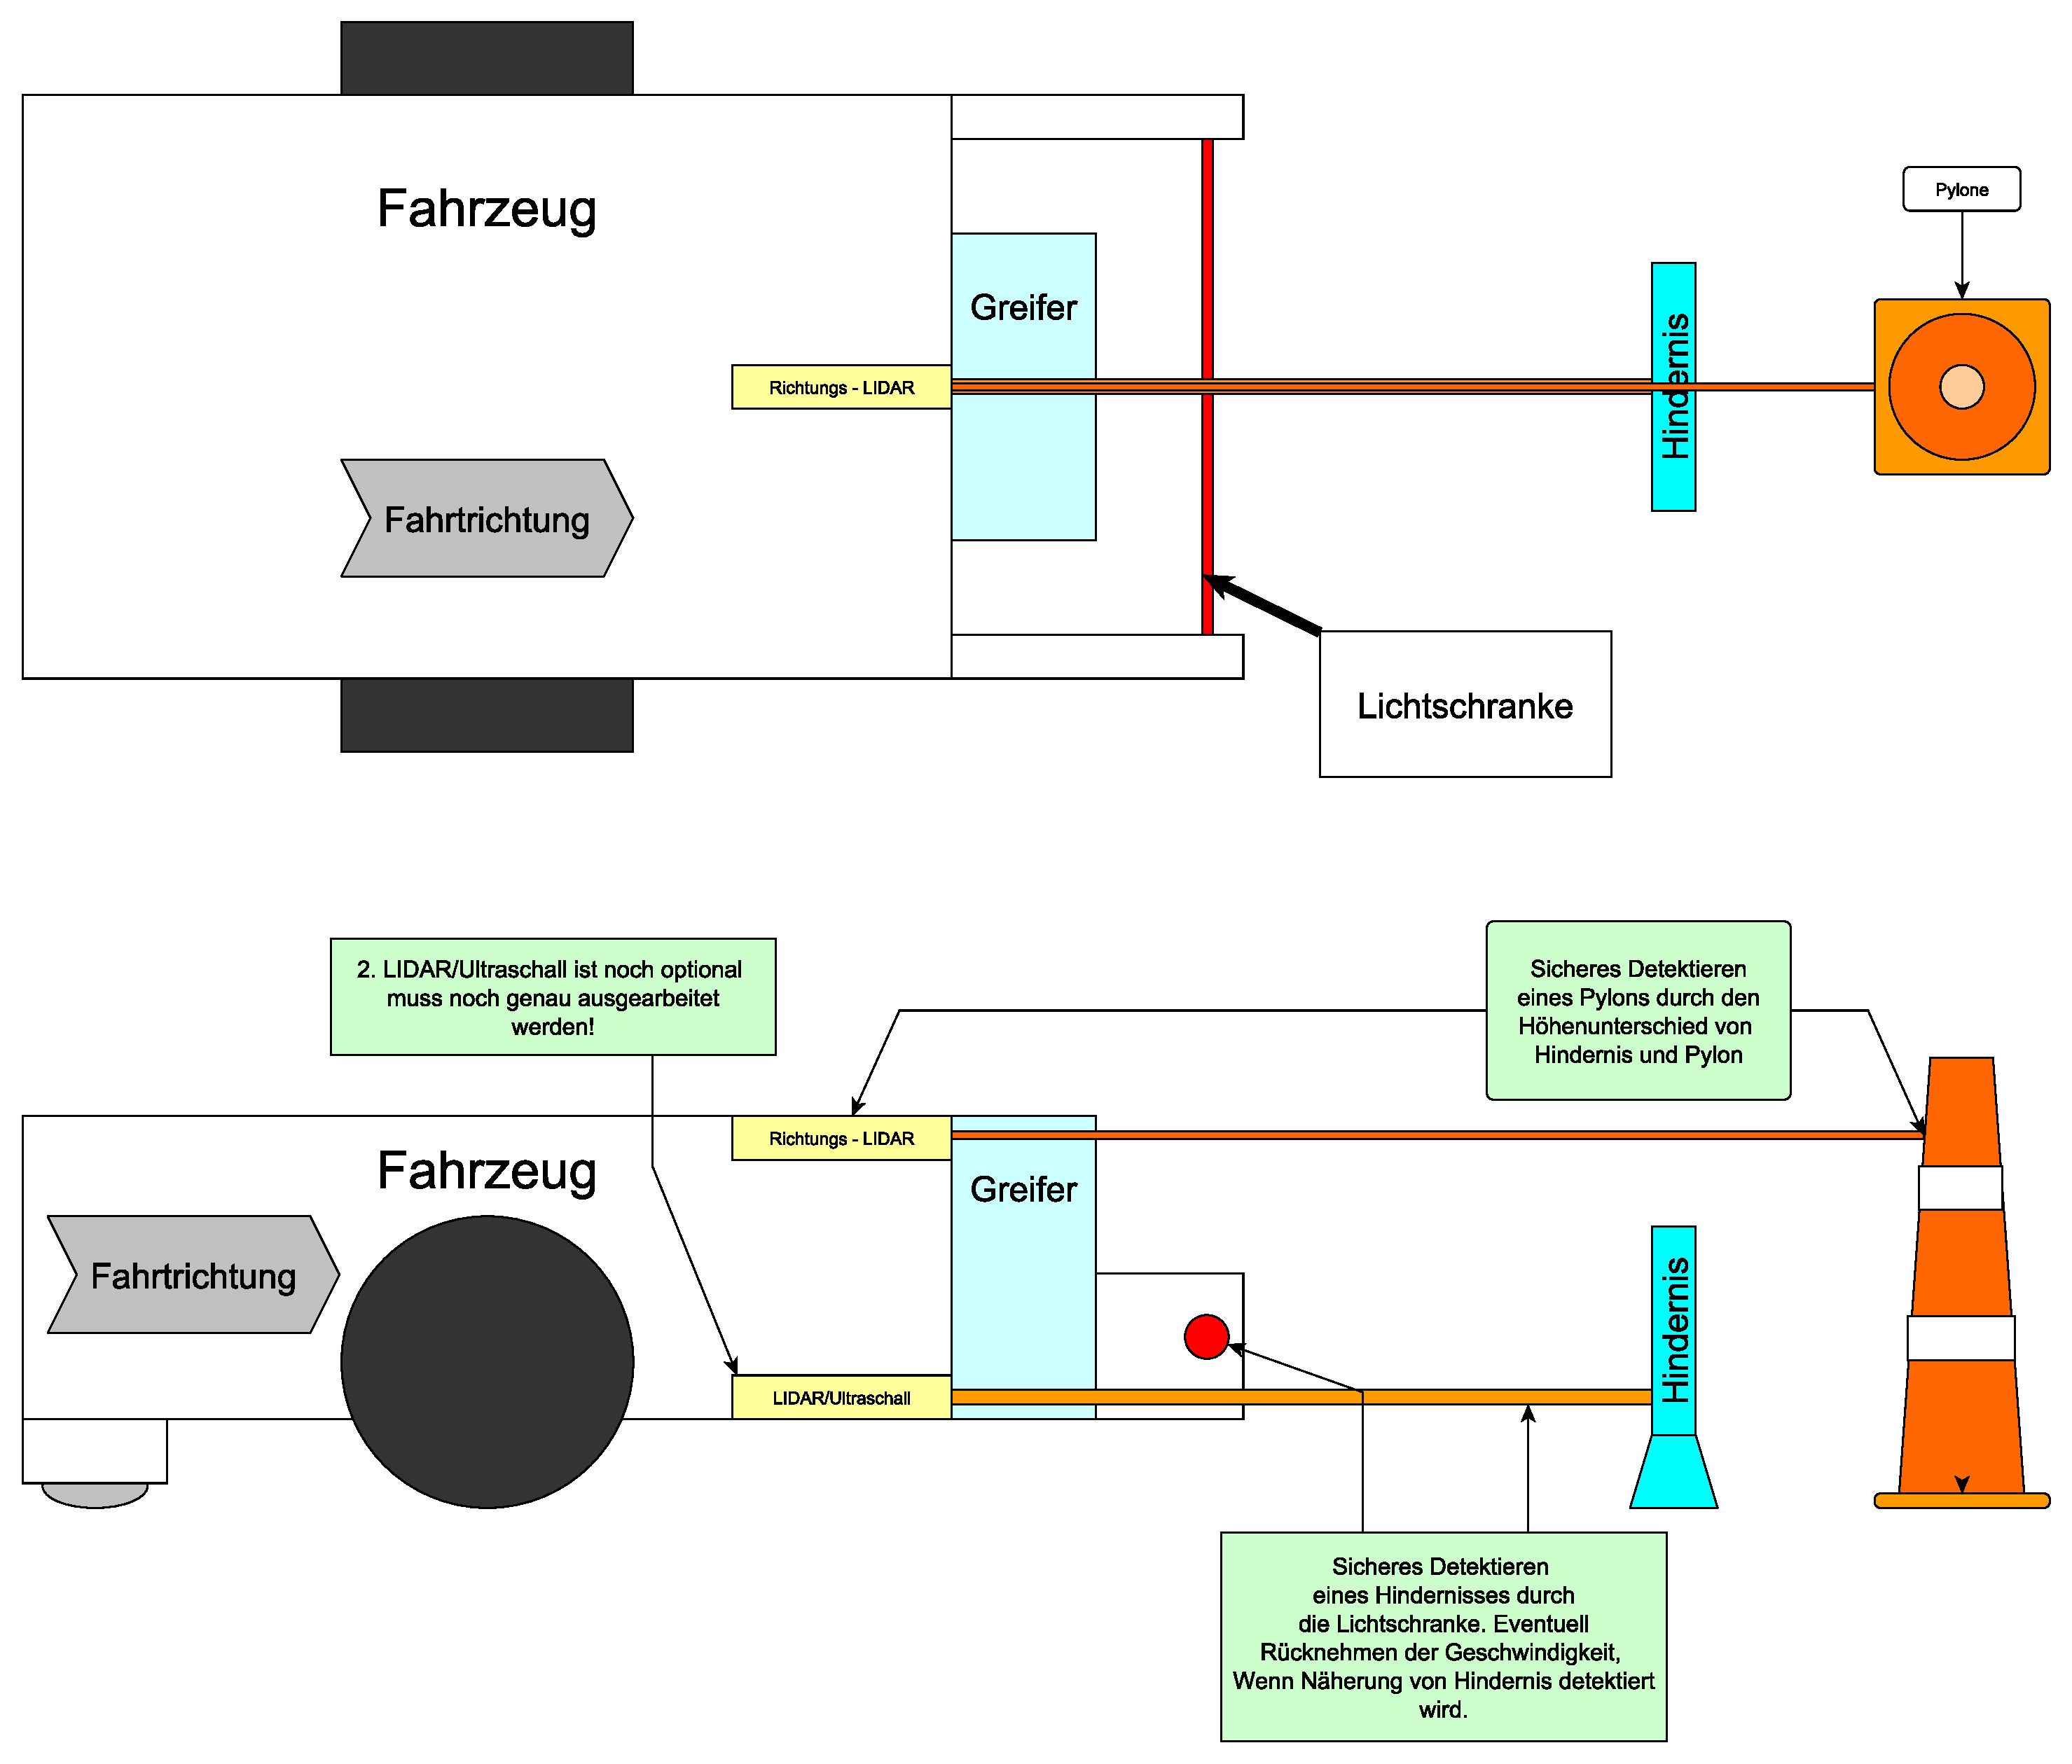
\includegraphics[width=0.75\linewidth]{./fig_Abstandssensor/Konzept_Hinderniserkennung.pdf}
    \caption{Konzept Hinderniserkennung}~\label{fig:Konzept_Hinderniserkennung}
\end{figure}

\paragraph{Eingesetzte Sensoren}
Verwendet wird der Ultraschallsensor \textit{HC-SR04}, sowie der
Richtungs-LIDAR \textit{TFLuna}.

\end{document}
